\section{Thermoelastic deformation in a hollow cylinder}
\subsection{Definition}

A hollow cylinder which consists of a solid of a constant temperature is exposed to a higher temperature at the surface of its hole. As a result of the increased temperature the cylinder is expanding. The aim of this calculation is to get out the radial displacement as well as the temperature distribution that are caused by the thermal expansion process by the use of an axisymmetric model. 
Figure \ref{fig68} shows a sketch of the calculation area assuming a homogeneous solid, a constant temperature in the whole body at the beginning and a heating of the cylinder at the inner surface.
Linear elastic material behaviour and isotropic thermal expansion are assumed. Deformations in $y$-direction at the bottom and the top and in $x$-direction at the right border are suppressed. The used parameters of the solid are listed in Table \ref{tab63}.

\begin{figure}[htbp]
\centering
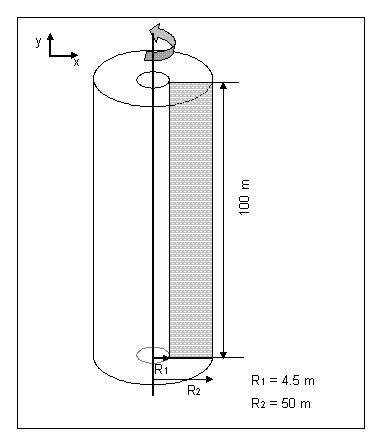
\includegraphics[width=0.45\textwidth]{PART_III/TM/figures/fig68}
\caption{Calculation area (grey area)}
\label{fig68}
\end{figure}

\begin{table}[htbp]
\centering
\caption{Model parameters}
\label{tab63}
\begin{tabular}{llrr}
\toprule
Symbol & Parameter & Value & Unit \\
\midrule
$T_0$  & Initial temperature (before heating) & 25 & $^{\circ}C$ \\
$q$  & Heat source & 30 & $W/m^2$ \\
$\rho$  & Density of the solid &  2000 & $kg \cdot m^{-3}$  \\			
$E$ & Young's modulus of the solid & 2.5 & $GPa$ \\
$\nu$ & Poisson ratio & 0.25 & $-$ \\
$\alpha$ & Thermal expansion & 4.2$\cdot$10$^{-5}$ & $K^{-1}$ \\
$\lambda$ & Thermal conductivity & 5.5 & $W\cdot m^{-1}\cdot K^{-1}$ \\
\bottomrule
\end{tabular}
\end{table}


%\textsl{Assumptions}
%
%\begin{tabbing}
%\=xxxxxxxxxxxx  \=xxxxxxxxxxxxxxxxxxxxxxx \kill
%\> Temperature: \> constant temperature in the whole body at the beginning, heating \\
%\> \> of the cylinder at the inner surface \\[1.0ex]
%\> Solid: \> homogeneous, finite dimensions, no deformation in $y$-direction at \\
%\> \> the bottom and the top, no deformation in $x$-direction at the right \\
%\> \> border, linear elastic material behaviour, isotropic thermal expansion
%\end{tabbing}

\subsection{Solution}
\subsubsection{Analytical solution} % WW derived the solution
For the hollow cylinder with the inner radius $R1$ and the outer radius $R2$ the following analytical solution for radial displacement $u_r$, stress $\sigma_r$ and temperature in dependency on the radius was used.% (Wang II, 2007).
\begin{eqnarray}
u_r & = &
\frac{q\,R_1\,\beta}{2\,\psi\,\kappa}\cdot r\cdot
\left(\ln\,r-\frac{1}{2}\right)\,+\,
\frac{A_0}{2}\,r\,+\,
\frac{A_1}{r}
\label{eq610} \\[2.0ex]
\sigma_r & = &
\psi\left[
-\frac{q\,R_1\,\beta}{2\,\psi\,\kappa}\cdot r\cdot
\left(\ln\,r+\frac{1}{2}\right)\,+\,
\frac{A_0}{2}\,-\,
\frac{A_1}{r^2}
\right] \nonumber \\[1.5ex]
 & & +\,
\lambda\left[
-\frac{q\,R_1\,\beta}{2\,\psi\,\kappa}\cdot r\cdot
\left(\ln\,r-\frac{1}{2}\right)\,+\,
\frac{A_0}{2}\,+\,
\frac{A_1}{r^2}
\right] \nonumber \\[1.5ex]
& & -\,\beta\left[
\frac{R_1\,q}{\kappa}\,\ln\left(\frac{R_2}{r}\right)\,+\,T_0
\right]
\label{eq611} \\[2.0ex]
T(r) & = &
\frac{R_1\,q}{\kappa}\,\ln\left(\frac{R_2}{r}\right)\,+\,T_0
\label{eq612}
\end{eqnarray}
{\small
where
\begin{displaymath}
\psi\,=\,\lambda\,+\,2\,G\qquad\mathrm{and}\qquad
\beta\,=\,\alpha\left(3\,\lambda\,+\,2\,G\right)
\end{displaymath}
with
\begin{tabbing}
\=xxxxxx \=xxxxxxxxxxxxxxxxxxxxxxxxxxxxxxxxx  \kill
\> $\lambda$   \> -- Lam$\acute{\mathrm{e}}$ elastic constant \\[0.5ex]
\> $G$         \> -- shear modulus \\[0.5ex]
\> $\alpha$    \> -- thermal expansion coefficient \\[0.5ex]
\> $\kappa$    \> -- thermal conductivity \\[0.5ex]
\> $A_0,\,A_1$ \> -- integration constants
\end{tabbing}
}

At the outer surface of the hollow cylinder (where $r=R_2$) there is no deformation, that means the displacement $u_{R2}$ is zero. Therefore equation \eqref{eq610} is set equal to zero for this boundary and adapted to $A_0$.
\begin{equation}
A_0\,=\,-\frac{2\,A_1}{R^2_2}\,-\,2\cdot B\cdot
\left(\ln\,R_2\,-\,\frac{1}{2}\right)
\label{eq613}
\end{equation}
{\small
where
}
\begin{displaymath}
B\,=\,\frac{q\,R_1\,\beta}{2\,\psi\,\kappa}
\end{displaymath}

At the inner surface of the hollow cylinder (where $r=R_1$) no stress is effected by the expansion because this boundary is phreatic. Therefore equation \eqref{eq611} is set equal to zero and $A_1$ is calculated by using equation \eqref{eq614}.
{\small
\begin{equation}
A_1=
\frac{
 \beta\!\left(\frac{
 \textstyle{R_1\,q}}{\textstyle{\kappa}}
 \ln\!\left(\frac{\textstyle{R_2}}{\textstyle{r}}\right)+T_0\right)
 \!+\!
 \lambda B\!\left(\ln R_1\!-\!\frac{1}{2}\right)\!+\!
 \psi B\!\left(\ln R_1\!+\!\frac{1}{2}\right)\!-\!
 \left(\frac{\textstyle{\lambda\!+\!\psi}}{\textstyle{2}}\right)
 2B\left(\ln R_2\!-\!\frac{1}{2}\right)
}
{\frac{
 \textstyle{\lambda-\psi}}{\textstyle{R^2_1}}-
 \frac{\textstyle{\lambda+\psi}}{\textstyle{2}}\cdot
 \frac{\textstyle{2}}{\textstyle{R^2_1}}\cdot
}
\label{eq614}
\end{equation}
}
After having solved this equation, $A_1$ is used to calculate $A_0$.




\subsubsection{Numerical solution}
The axisymmetric model is in the $xy$-plane. The inner radius $R1$ of the cylindrical model is 4.5~m and the outer radius $R2$ 50~m. The cylinder is 100~m high. The initial temperature in the whole area is 25$^{\circ}$C. As boundary condition deformations in $y$-direction at the bottom and the top are suppressed, as well as deformations in $x$-direction at the right border. At the right boundary of the model a thermal boundary condition is set with a constant value of 25$^{\circ}$C. At the left boundary a source term for heat flux of $q=30$~W/m$^2$ is defined. Thereby the continuous heating of the solid is simulated.  The simulation of only one time step is done. The numerical model consists of 766 triangular elements and 426 nodes as sketched in Figure \ref{fig69}.

\begin{figure}[htbp]
\centering
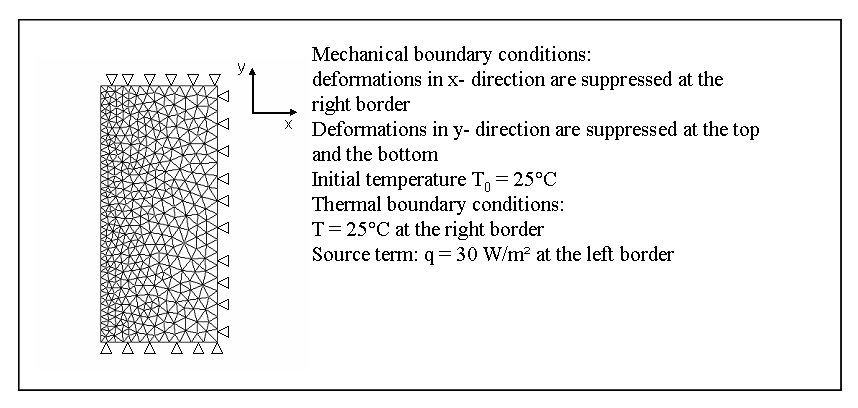
\includegraphics[width=0.6\textwidth]{PART_III/TM/figures/fig69.eps}
\caption{Mesh for TM coupling hollow cylinder model (2D axisymmetric)}
\label{fig69}
\end{figure}

\begin{figure}[htbp]
\centering
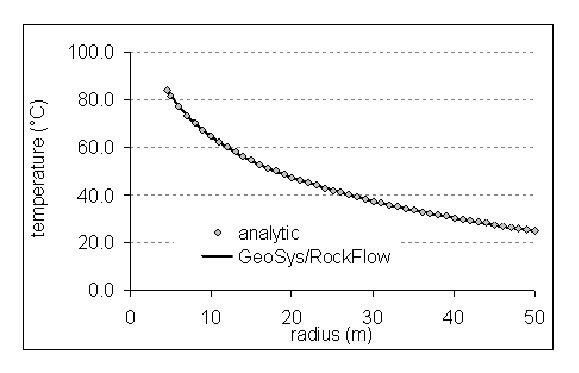
\includegraphics[width=0.7\textwidth]{PART_III/TM/figures/fig610}
\caption{Temperature distribution over the radius}
\label{fig610}
\end{figure}

\begin{figure}[htbp]
\centering
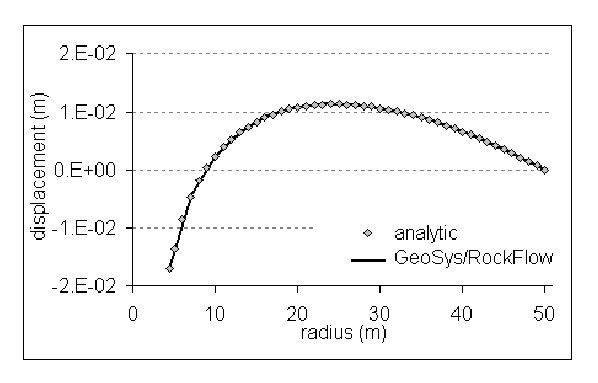
\includegraphics[width=0.7\textwidth]{PART_III/TM/figures/fig611}
\caption{Displacements in radial direction}
\label{fig611}
\end{figure}

\begin{figure}[htbp]
\centering
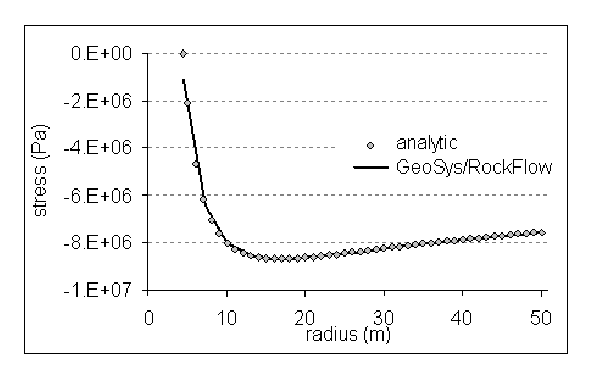
\includegraphics[width=0.7\textwidth]{PART_III/TM/figures/fig612}
\caption{Stresses in radial direction}
\label{fig612}
\end{figure}

\subsection{Results}
The results of the analytical equations for stresses, displacements and temperatures are compared to those of the numerical simulation by OGS. 
With the equations \eqref{eq614} and \eqref{eq613} and the used parameters, the integration constants in the analytical solution are obtained as: 
\begin{eqnarray*}
A_0 & = & \phantom{-}5.96\cdot10^{-3} \\[1.0ex]
A_1 & = & -1.19\cdot10^{-1}
\end{eqnarray*}

Figure \ref{fig610} shows the temperature distribution over the radius of the hollow cylinder. In Figure \ref{fig611} displacements in radial direction that are caused by the thermal expansion are depicted. In addition you can find the induced stresses in Figure \ref{fig612}. Obviously, with the axisymmetric model a OGS simulation generates comprehensible results that meet well the analytic solution.